\errorcontextlines=9999
\documentclass[
   aspectratio=169, % default is 43
   10pt, % font size, default is 11pt
   % nosectionframes,
   uniqueslidenumber,
   % handout,
   professionalfonts
]{beamer}

\usepackage[T1]{fontenc}
\usepackage[utf8]{inputenc}
\usepackage[sfdefault]{FiraSans}

\usepackage{stmaryrd}
\usepackage[vvarbb]{notomath}
\usepackage{FiraMono}
\usepackage{tikz,forest}
\usepackage{fontawesome}
\usepackage{csquotes}
\usepackage{relsize}
\usepackage{simplebnf}
\usepackage{../abstract-interpretation-ltx/absint}
\makeatletter
\def\absint@reflab#1#2{#2}% we do not need labels here
\usetikzlibrary{arrows.meta,decorations.pathmorphing,fit,decorations.pathreplacing,backgrounds,matrix}
\pgfdeclarelayer{foreground}
\usepackage[glows]{tikzpingus}
\pgfsetlayers{very-background,background,main,middle,foreground}
\def\sbseries{\fontseries{sb}\selectfont}
\def\textsb#1{{\sbseries#1}}
\tikzset{bottom note/.style={font=\scriptsize,scale=.8,color=gray}}
\usepackage{../slide-template-uulm/fancybeamer} % use the fancy beamer package
\usepackage{../slide-template-uulm/fancyuulm}
\setpaths{{../slide-template-uulm/}{../slide-template-uulm/logos/}{../slide-template-uulm/empty-slides/}{../xlistings/}}

\usepackage{../code-animation/code-animation}
\usepackage[fakeminted,print]{../xlistings/xlistings}
\usepackage{multirow}
\xlstsetmintedstyle{plain}
\LoadLanguages{R,Java}
\lstcolorlet{keywordA}{black!70!red}%
\lstcolorlet{keywordB}{black!70!red}%
\lstcolorlet{keywordC}{black!70!red}%
\lstcolorlet{numbers}{black!70!yellow}%
\def\absintstyle#1{#1}

% bib
\usepackage[style=alphabetic,backend=biber]{biblatex}
\addbibresource{./references.bib}

\title{Static Analysis in the Real World}
\subtitle[SQA]{Software Quality Assurance - Static Code Analysis, III}
\author[F. Sihler]{Florian Sihler}
\date{\today} % use a particular date here if needed

\fancylogos{sp,uulm} % define logos that are spread evenly across the bottom of the title slide

\usepackage{../beamer-latex-pdfpc-notes}

\begin{document}

\maketitle[titleimage/title][40]

\mode
<handout>

\begin{frame}{Outline}
% \begin{multicols}{2}
\tableofcontents[hideallsubsections]
% \end{multicols}
\end{frame}

\mode
<all>

\newsavebox\abstractionbox
\begin{lrbox}{\abstractionbox}
\begin{tikzpicture}[line cap=round]
   \pgfonlayer{foreground}
   \draw[Kite-Kite,very thick] (0,3.5) node[below right,yshift=1mm] {\(x(t)\)} |- (8,0) node[above left] {\(t\)}; % time vs. x at tat time
   \endpgfonlayer
   \colorlet{@}{gray}
   \draw[very thick,@] (0,1) plot [smooth] coordinates {(0,1) (1,2) (2,1) (3,2) (4,1) (5,2) (6,1) (7,2) (8,1)}; % x(t)
   \draw[very thick,@] (0,0) plot [smooth] coordinates {(0,0) (1,1) (2,2) (3,2) (4,2.5) (5,2.5) (6,.5) (7,.6) (8,.6)}; % x(t)
   \draw[very thick,@] (0,1.5) plot [smooth] coordinates {(0,1.5) (1,2) (2,2.5) (3,2) (4,2) (5,2.5) (6,2.5) (7,2) (8,2.5)}; % x(t)
      \foreach \i in {0,...,5} {
         \pgfmathsetmacro{\randA}{rnd*0.33}
         \pgfmathsetmacro{\randB}{rand*0.5}
         \pgfmathsetmacro{\randC}{rand*0.4}
         \draw[gray] (0,1.5+\randA) plot [smooth] coordinates {(0,1.5+\randA) (1,2-\randB) (2,2.5-\randA) (3,2-\randB) (4,2+\randA) (5,2.5) (6,2.5+\randA) (7,2-\randA) (8,2.5+\randB)} node[inner sep=0pt] (a-\i) {};
         \draw[gray] (0,0+\randA) plot [smooth] coordinates {(0,0+\randA) (1,1-\randB) (2,2-\randB) (3,2+\randC) (4,2.5-\randA) (5,2.5-\randB) (6,.5+\randC) (7,.6+\randB) (8,.6+\randC)} node[inner sep=0pt] (b-\i) {};
         \draw[gray] (0,1+\randB) plot [smooth] coordinates {(0,1-\randC) (1,2-\randB) (2,1+\randB) (3,2-\randA) (4,1+\randA) (5,2-\randB) (6,1) (7,2-\randC) (8,1+\randA)} node[inner sep=0pt] (c-\i) {};
      }
   % fit to all nodes to get the bounding box
   \node[fit=(a-0) (a-1) (a-2) (a-3) (a-4) (a-5) (b-0) (b-1) (b-2) (b-3) (b-4) (b-5) (c-0) (c-1) (c-2) (c-3) (c-4) (c-5),inner sep=0pt] (big-ghost) {~};
      % \draw[decorate,thick,decoration={brace,amplitude=5pt,raise=2pt},gray] (big-ghost.north east) -- (big-ghost.south east);
   \pgfonlayer{background}
   \pgfinterruptboundingbox
   \fill[red,opacity=.175,even odd rule] plot [smooth] coordinates {(0,0) (1,0.4) (2,0.5) (3,1) (4,.8) (5,1) (6,.1) (7,0.2) (8.03,.2) (8.03,3) (7,2.8) (6,3) (5,2.95) (4,2.85) (3,2.75) (2,2.65) (1,2.5) (0,2) } -- cycle (6,1.85) circle[radius=4mm]; 
   \endpgfinterruptboundingbox
      \node (@b1) at (6,1.85) {\small\faBug};
      \node (@b2) at (3,.35) {\small\faBug};
      \node (@b3) at (7,2.5) {\small\faBug};
      \node[above left=-1mm,green] at(@b2.south east) {\scriptsize\faCheck};
      \node[above left=-1mm,green] at(@b1.south east) {\scriptsize\faCheck};
      \node[above left=-1mm,yshift=1pt,orange] at(@b3.south east) {\scriptsize\faQuestion};
   \endpgfonlayer
   \path[use as bounding box] (0,0) rectangle (8,3.5);
\end{tikzpicture}
\end{lrbox}

\begin{frame}{What we have\ldots}
\frametitle<-8>{\strut What we have\ldots}%
\frametitle<9->{\strut\textcolor{gray}{What we have\ldots~}Theory}%
\pgfmathsetseed{42}%
\begin{uncoverenv}<2->  
\begin{tikzpicture}[baseline={([yshift=-.5ex]current bounding box.center)},line cap=round]
   \tikzset{@/.style={opacity=1}}
   \def\scaler{1}
   \only<4->{\def\scaler{0.5}\tikzset{@/.style={opacity=.5,scale=.5,every node/.style={transform shape}}}}
   \scope[transparency group, @]
   \node (@) at (0,0) {\usebox\abstractionbox};
   \onslide<3>{
   \draw[decorate,thick,decoration={brace,amplitude=8pt*\scaler,raise=2pt},line width=0.5pt*\scaler] (@.north east) to[edge node={node [right=3.5mm] {Abstractions}}] (@.south east);
   }
   \onslide<4->{%
      \node[below] at(@.south) {Abstractions};
   }
   \endscope
\end{tikzpicture}
\begin{uncoverenv}<5->
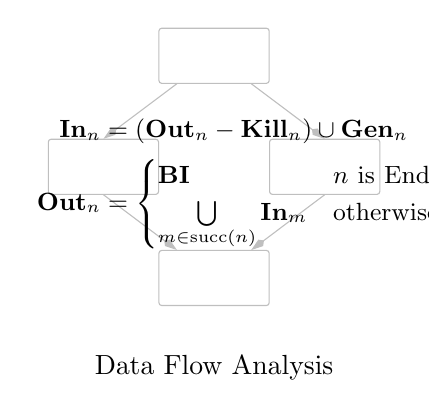
\begin{tikzpicture}[r/.style={rectangle,draw,minimum width=2cm,minimum height=1cm,rounded corners=1pt},baseline={([yshift=-.5ex]current bounding box.center)},line cap=round]
   \tikzset{@/.style={opacity=1}}
   \def\scaler{1}
   \only<7->{\def\scaler{0.5}\tikzset{@/.style={opacity=.5,scale=.5,every node/.style={transform shape}}}}
   \scope[@]
   \scope[black!25!white,scale=.7,every node/.style={transform shape}]
   \node[r] (@) at(0,0) {};
   \node[r, below left=1cm] (@a) at(@.south) {};
   \node[r, below right=1cm] (@b) at(@.south) {};
   \node[r,below=1cm] (@c) at(current bounding box.south) {};
   \draw[-Kite] (@) -- (@a.north);
   \draw[-Kite] (@) -- (@b.north);
   \draw[-Kite] (@a.south) -- (@c);
   \draw[-Kite] (@b.south) -- (@c);
   \endscope
   \node[align=center,text width=4.5cm] at(current bounding box.center) {\small%
\begin{align*}
   \mathbf{In}_n &= (\mathbf{Out}_n - \mathbf{Kill}_n) \cup \mathbf{Gen}_n \\
   \mathbf{Out}_n &= \begin{cases}
      \mathbf{BI} & n \text{~is End} \\
      \bigcup\limits_{m \in \text{succ}(n)} \mathbf{In}_m & \text{otherwise}
   \end{cases}
\end{align*}
   };
   \onslide<6->{
      \node[below=5mm] at(current bounding box.south) {Data Flow Analysis};
   }
   \endscope
\end{tikzpicture}
\end{uncoverenv}
\hspace*{4.5em}\onslide<8->{\large\ldots}
\end{uncoverenv}
\end{frame}

\newsavebox\CodeFile
\begin{lrbox}{\CodeFile}
\scalebox{1.45}{%

\begin{tikzpicture}
   \draw[rounded corners=1.5pt,fill=white] (0,0) |- ++(.6,-.8) [sharp corners] -- ++(0,.6) -- ++(-.2,.2) coordinate (@rl) [rounded corners=2pt] -- cycle (@rl) |- ++(.2,-.2);
   \draw[thick,line cap=round,lightgray] (.1,-.1) -- ++(.2,0)
      % for what have I written random code generation? :C 
      (.1,-.15) -- ++(.1,0) ++(.05,0) -- ++(.1,0)
      (.125,-.2) -- ++(.15,0)++(.05,0)--++(.025,0)
      (.1,-.25) -- ++(.3,0)
      (.125,-.3) --++(.2,0)++(.05,0)--++(.05,0)
      (.125,-.35) --++(.15,0)++(.05,0)--++(.1,0)
      (.15,-.4)--++(.2,0)
      (.15,-.4)--++(.1,0)++(.05,0)--++(.05,0)
      (.125,-.45)--++(.05,0)
      (.1,-.5)--++(.066,0)++(.05,0)--++(.15,0)
      (.1,-.6)--++(.15,0)++(.05,0)--++(.15,0)
      (.1,-.65)--++(.2,0)
      (.1,-.7)--++(.1,0)++(.05,0)--++(.15,0)
   ;
\end{tikzpicture}}
\end{lrbox}
\newsavebox\MagicPenguin
\savebox\MagicPenguin{\tikz{\pingu[witch hat,eyes wink,wings wave,bee,blush,santa beard]}}
\newsavebox\MagicPenguinTwo
\savebox\MagicPenguinTwo{\tikz{\pingu[witch hat,eyes shiny,bee,santa beard]}}
\begin{frame}{What we want\ldots}
   \frametitle<1>{What we want\ldots~}%
   \frametitle<2->{\textcolor{gray}{What we want\ldots~}Tools}%
   \centering\kern1.345em
   \begin{uncoverenv}<3->
   \begin{tikzpicture}[o/.style={outer sep=0pt,inner sep=0pt},line cap=round,Rect/.style={draw,rectangle,rounded corners=3pt,inner sep=4pt,outer sep=1mm},draw=gray,every path/.append style={thick}]
      \node[o] (@) at (0,0) {\usebox\CodeFile};
      \pgfonlayer{background}
      \scope[transparency group,opacity=.4]
      \node[o,rotate around={-30:(@.south east)},anchor=south east] at(@.south east) {\usebox\CodeFile};
      \node[o,rotate around={-12:(@.south east)},anchor=south east] at(@.south east) {\usebox\CodeFile};
      \endscope
      \endpgfonlayer
      \node[below] at(@.south) {\small Project};
      \onslide<3->{
         \node[right=1.33cm,Rect,minimum width=4.5em] (@magic) at(@.east) {~\vphantom{Magic}{\only<8->{\only<9->{\color{gray!34}}\clap{Magic}}}\only<9->{\clap{\kern-.8pt\textbf{Tools}}}~\null};
         \draw[-Kite] ([xshift=5mm]@.east) -- (@magic.west);
      }
      % and how can we achieve that?... magic :sparkles: but as there is no magic, we need tools... and algorithms
      \onslide<8->{
         \node[above right,xshift=1.3mm] at(@magic.north west) {\scalebox{.45}{\only<-8|handout:0>{\kern-8.5pt\usebox\MagicPenguin}\only<9->{\usebox\MagicPenguinTwo}}};
      }
      \coordinate (@) at(@magic.east);
      \foreach[count=\i] \usecase/\targeti in {Security/4, Maintenance/5, Comprehension/6, Optimization/7, Usability/7, \ldots/7} {
      \pgfmathsetmacro\rot{-11*\i+38.75}
         \onslide<\targeti->{
            \node[right=1cm,Rect,rotate around={\rot:([xshift=-9mm]@.east)},minimum width=8em,fill=white] (@uc-\i) at (@.east) {\strut\usecase};
            \draw[-Kite,sharp corners] (@.east) -- ++(4.2mm,0) [rounded corners=1pt] arc (0:\rot:9mm) -- (@uc-\i.west);
         }
      }
      \onslide<11->{
         \scope[gray]
         \node[right] at (@uc-1.east) {\small injections, leaks,~\ldots};
         \node[right] at (@uc-2.east) {\small code clones, deprecation,~\ldots};
         \node[right] at (@uc-3.east) {\small documentation, structure,~\ldots};
         \node[right] at (@uc-4.east) {\small better algorithms, memoization,~\ldots};
         \node[right] at (@uc-5.east) {\small color deficiency, size,~\ldots};
         \node[right] at (@uc-6.east) {\small \only<-11|handout:0>{\ldots}\only<12->{architecture recovery, refactoring,~\ldots}};
         \endscope
      }
      \onslide<13->{
         \draw[Kite-] (@magic.south) -- ++(0,-.66) node[below,align=center,font=\footnotesize] {SonarQube\rlap{\textsuperscript{1}}, Teamscale\rlap{\textsuperscript{2}},\\lintr\rlap{\textsuperscript{3}}, CodeQL\rlap{\textsuperscript{4}}, \ldots};
      }
   \end{tikzpicture}

   \begin{tikzpicture}[overlay,remember picture]
      \onslide<10->{%
         \node[above=9mm,lightgray] at(current page.south) {\footnotesize\enquote{Any sufficiently advanced technology is indistinguishable from magic.} --- Arthur C. Clarke};% 3rd law
      }
      \onslide<13->{\node[bottom note,above right,yshift=5mm] at(current page.south west) {%
         \textsuperscript{1}\,\href{https://www.sonarsource.com/}{sonarsource.com}, \textsuperscript{2}\,\href{https://teamscale.com/}{teamscale.com}, \textsuperscript{3}\,\href{https://lintr.r-lib.org/}{lintr.r-lib.org}, \textsuperscript{4}\,\href{https://codeql.github.com/}{codeql.github.com}%
      };}
   \end{tikzpicture}
   % TODO: tool examples
   % rather list concrete problems than tools
\end{uncoverenv}
\end{frame}

\begin{frame}{What do they\ldots~do?}
% they take input, textual, syntactical, semantic (call graphs, pdg, ...), metadata, historical information, requirements, annotations (types, contracts), ...

\begin{tikzpicture}[o/.style={outer sep=0pt,inner sep=0pt}]
   \onslide<2->{%
      \node[o] (@) at (0,0) {\usebox\CodeFile};
      \node[above=2.5mm,xshift=1.15mm,gray] at(@.north) {\tiny They take \textbf{\normalsize Input}};
   }
   \pgfonlayer{background}
   \onslide<2->{%
   \scope[transparency group,opacity=.4]
   \node[o,rotate around={-30:(@.south east)},anchor=south east] at(@.south east) {\usebox\CodeFile};
   \node[o,rotate around={-12:(@.south east)},anchor=south east] at(@.south east) {\usebox\CodeFile};
   \endscope}
   \endpgfonlayer
   \begin{uncoverenv}<3->
   \coordinate (@) at(@.east);
   \foreach[count=\i] \usecase/\targeti in {{\raisebox{1pt}{Textual}}/4,Syntactical/5, Semantical/6, Historical/7, Annotations/8, {\only<-9|handout:0>{\ldots}\only<10->{\raisebox{-3pt}{Metadata,~\ldots}}}/9} { % program spectra, hardware, contexts, ...
   \pgfmathsetmacro\rot{-24*\i+66}
      \onslide<\targeti->{
         \path ([xshift=.5mm]@.east)++(\rot+10:1mm) coordinate (@a);
         \fill[opacity=.18,gray] (@a.east) -- ++(\rot:1.5cm) arc (\rot:\rot+20:1.5cm) -- cycle;
         \draw[thick,gray] (@a.east)++(\rot:1.5cm) arc (\rot:\rot+20:1.5cm);
         \path (@a.east) -- ++(1.05*\rot+10:1.6cm) node[right,font=\small,darkgray] {\vphantom{a}\smash{\usecase}};
      }
   }
   \node[above=1.65mm,xshift=1mm,gray] at(current bounding box.north) {\tiny And use \textbf{\normalsize Perspectives} \rlap{(often combined)}};
   \end{uncoverenv}
   \onslide<11->{%
      \draw[Kite-,gray] ([xshift=7.5mm]current bounding box.south) to[out=-90,in=0] ++(-3mm,-5mm) node[below left,yshift=.7\baselineskip,align=right,text width=2.5cm,font=\tiny] {Some of those are the result of other static or dynamic analyses};
   }
   \begin{uncoverenv}<11->
      \node[right,yshift=-5mm,xshift=1cm,align=left,font=\small,darkgray,text width=3.5cm] (@techn) at(current bounding box.east){Text Search\\[4mm]{\onslide<12->{Clustering}}\\[4mm]{\onslide<13->{Abstract Domains}}\\[4mm]{\onslide<14->{Dataflow Constraints}}\\[3mm]{\onslide<15->{\centerline{\(\vdots\)}}}};
      \onslide<16->{
         \node[below,gray,xshift=-4.5mm] at(@techn.south) {\tiny Together with \textbf{\normalsize Theory}};
      }
   \end{uncoverenv}
\end{tikzpicture}
\end{frame}

\begin{frame}
   Wir hatten Abstraktionen, Theorie, jetzt mal mehr wie das abläuft
   ~> Programm rein, CFG, Basic Blocks, AST, analysis passes, completeness vs. soundness
\end{frame}

\begin{frame}
   Tabelle mit astree, sonar lint cube, lintr, .. aber eben auch nicht fehlerfinden sondern z.b. globals, renaming, etc.
\end{frame}

\begin{frame}
   TODO: dynamic analysis alternative
\end{frame}

% \section{The Why}
% \subsection[Motivation]{Initial Motivation}
% \begin{frame}[fragile,label=main-example]{\insertsection}
% x
% \end{frame}

\renewcommand*{\bibfont}{\tiny}

\AtBeginSection{}
\begin{frame}[allowframebreaks]{References}
   \printbibliography[title={}] % TODO
\end{frame}

\end{document}